\section{Smart City and Indoor Positioning Systems} % 28-32 Seiten

\subsection{Definition of the Term Smart City} 
To derive a definition of the term Smart City at first the question "What is a city?" is answered. After that a closer look to the "Smart" City is taken. A formal definition is provided at the end of this section.
 
\subsubsection{What is a city?}
The first urban settlements evolved more than 5000 years ago in the two great civilizations of Mesopotamia and Egypt \parencite{berUrban}. Much later in the fourteenth century with entry into the world urban system of the capitals of nation states and the centers of international trade urban settlements began to grow much faster than before \parencite{urbanTrends}. However, this leads to the first approach to define a city as as an Urban Area which is an area of continuous urban development which includes the historical core municipality, and the adjacent suburbs. 
Changing the perspective to the government we can also define a city as a municipality or local authority area which was done so by the International Organization for Standardization in the ISO 37120 where the city is defined as "urban community falling under a specific administrative boundary, commonly referred to as a city, municipality or local government" \parencite{ISO37120}. %https://www.iso.org/obp/ui/#iso:std:iso:37120:ed-1:v1:en
As a third perspective a more mathematical approach for a definition was provided by the European Commission:

\begin{figure}[h]
	\centering
		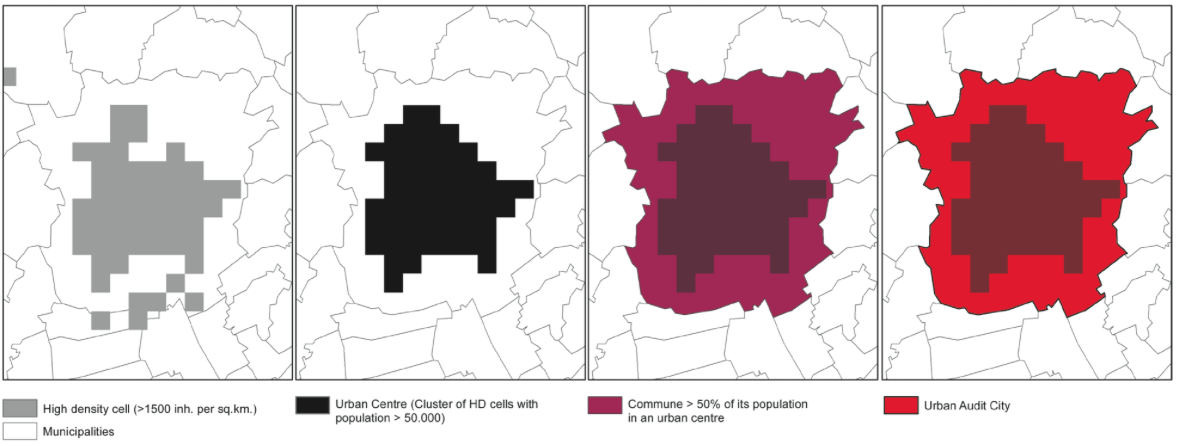
\includegraphics[width=.9\textwidth]{images/graz.png}
	\caption{High density cells, urban centre and city (Graz) \parencite{euDef}}
	\label{fig:images_graz}
\end{figure}

"Step 1: All grid cells with a density of more than 1 500 inhabitants per sq km are selected (\ref{fig:images_graz}.1).
Step 2: The contiguous (2) high-density cells are then clustered, gaps (3) are filled and only the clusters with a minimum population
of 50 000 inhabitants (\ref{fig:images_graz}.2) are kept as an ‘urban centre’.
Step 3: All the municipalities (local administrative units level 2 or LAU2) with at least half their population inside the urban centre are selected as candidates to become part of the city (\ref{fig:images_graz}.3).
Step 4: The city is defined ensuring that 1) there is a link to the political level, 2) that at least 50 \% of city the population lives in an urban centre and 3) that at least 75 \% of the population of the urban centre lives in a city (\ref{fig:images_graz}.4) (4)" "\parencite{euDef}.

Due to the fact that we consider Smart City projects not limited to a municipality or local authority area, or the strict constrains as given in the last described approach, a definition of a city as urban area is used for later work.
 
\subsubsection{\textit{Definition: City}}
The City as Urban Area includes the "urban community falling under a specific administrative boundary, commonly referred to as a city, municipality or local government" \parencite{ISO37120}, the adjacent suburbs as well as the exurbs being under continuous urban development driven by the central municipality or local government.

\subsubsection{What makes a City Smart?}
According to \textcite{networkedCities} the main smart city characteristics are the use of digital infrastructure, information and communication technologies (ICT), the emphasis of business-led urban development (which results in characteristics the Central of Regional Science at the Vienna University of Technology (2007) calls a smart economy), the social inclusion agenda via the use of e-governance and urban sustainability  \parencite{networkedCities}. 

The motivation for Smart City projects is represented by the urbanization which requires a more efficient, effective and reliable usage of the cities infrastructure \parencite{berUrban}. The goal is to improve economic and political efficiency at the same time to enable social, cultural and urban development. Which implies a community whose members have to learn adapt and innovate. To archive that the concept includes attracting creative individuals to cities in order to help stimulate urban growth \parencite{networkedCities}. This aspect of smart cities being creative cities is also considered by \textcite{persSmart} stating that smart cities are "seedbeds for creativeness, innovation, entrepreneurship and spatial competitiveness". 

However, there is not one general definition for a Smart City, and the number of publications with the topic Smart City was 152 only in 2012 \parencite{smartCity}. That is why we decided to recite 6 of the most cited definitions collected during a review of literature in \textcite{smartCity}. The other definitions given in that paper are listed in the appendix. 

\subsubsection{\textit{Definitions: Smart City}}

\begin{quote}[\textcite{smart2}]
“A smart community is a community that has made a conscious effort to use information technology to transform life and work within its region in significant and fundamental rather than incremental ways.” \end{quote}

\begin{quote}[\textcite{smart3}]
“A city to be smart when investments in human and social capital
and traditional (transport) and modern (ICT) communication infra- structure fuel sustainable economic growth and a high quality of life, with a wise management of natural resources, through participatory governance.” 
\end{quote}

\begin{quote}[\textcite{smart4}]
“Smart city is defined by IBM as the use of information and communication technology to sense, analyze and integrate the key information of core systems in running cities.” 
\end{quote}

\begin{quote}[\textcite{smart7}]
“A city that monitors and integrates conditions of all of its critical infrastructures, including roads, bridges, tunnels, rails, subways, airports, seaports, communications, water, power, even major buildings, can better optimize its resources, plan its preventive maintenance activi- ties, and monitor security aspects while maximizing services to its citizens.”
\end{quote}

\begin{quote}[\textcite{smart8}]
“Smart City is a city in which it can combine technologies as diverse
as water recycling, advanced energy grids and mobile communications in order to reduce environmental impact and to offer its citizens better lives.”
\end{quote}

\begin{quote}[ \textcite{smart9}]
“A smart city is a well-defined geographical area, in which high technolo- gies such as ICT, logistic, energy production, and so on, cooperate to create benefits for citizens in terms of well-being, inclusion and participation, environmental quality, intelligent development; it is governed by a well-defined pool of subjects, able to state the rules and policy for the city government and development.” 
\end{quote}

All this definitions intersect each other, but are not always coincident. For our purpose we decided that the definitions of \textcite{smart9} and \textcite{smart4} are underlining our view on Smart Cities precisely. To clarify our position we will outline some characteristics every smart city has. Since we do not want to define a city as smart in case of perfect monitoring and survailliance \textcite{smart7} is not our view on a smart city. We want to define smart city in the eyes of the user to enable the most benefit.  

\subsubsection{Smart City in Detail}
Everything being part of a city is affected by the goal of a city to be Smart. Some more than others, but still there will be a noticeable change. The six main characteristics and factors of Smart Cities collected by \textcite{smartCharacter} can help to correlate Positioning Systems with the purpose of Smart Cities. These characteristics are Smart Economy - which is the competitiveness between different cities, Smart Governance - which is measured by the possibility of participation by the citizens, Smart Environment - which is the sustainable management of natural resources, Smart People - which are the social component in Smart Cities, Smart Mobility - which is the way of Transportation and use of ICT and Smart Living - which affects the quality of life influenced by Smart Home. All this is shown in more detail in figure \ref{fig:characteristics}. 
Indoor positioning can be ranged in smart mobility as providing availability of ICT infrastructure and smart living (quality of life) in case of cultural facilities. 

\begin{figure}[h]
	\centering
		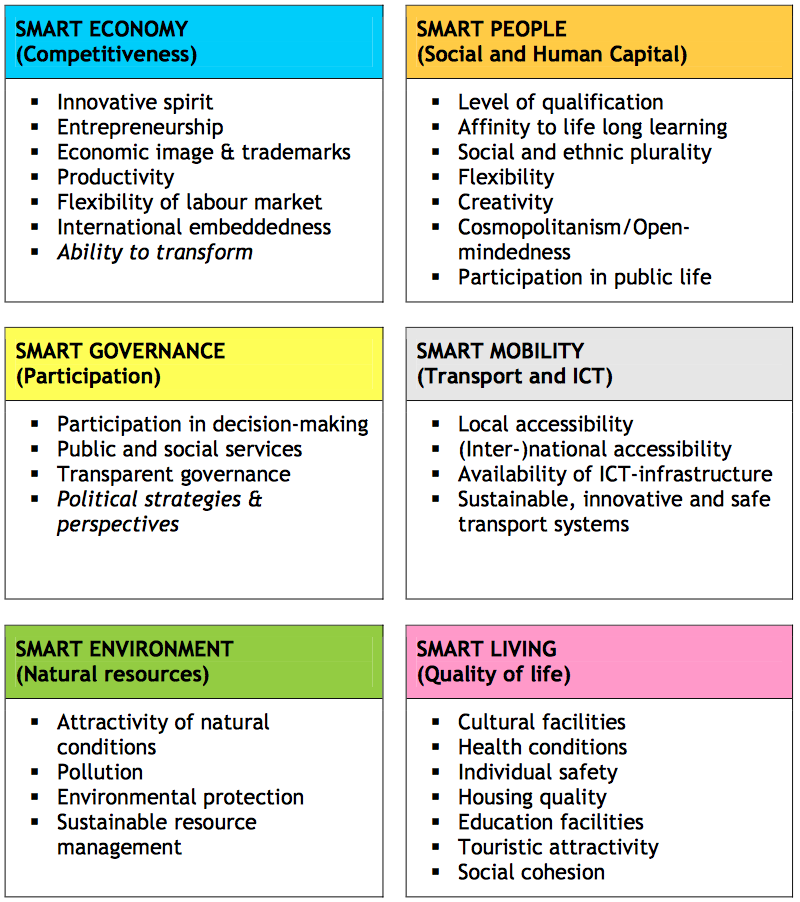
\includegraphics[width=.9\textwidth]{images/characteristics.png}
	\caption{Characteristics and factors of Smart Cities \parencite{smartCharacter}}
	\label{fig:characteristics}
\end{figure}

Positioning Systems in Smart Cities will hopefully increase the quality of life by providing additional ICT-infrastructure. 

\subsection{Positioning in Smart Cities}\label{posInCS}
The first tools for navigation have been especially developed for sailors. Now in our century we encounter numerous navigation and positioning systems in our everyday lives. For example the automotive navigation systems in our cars, or the navigation and positioning systems in our smartphones. These applications mostly use Global Positioning System (GPS) to determine their location. Some of them are using Wi-Fi to precise the localization. These commonly used navigation systems have displaced paper street maps for many users. But taking a look at our every day behavior there are still places we have to look out for maps. All these places are potential areas for indoor navigation systems. 

In the following section some use cases should make this need for indoor positioning in the context of Smart City even more comprehensible.

\subsubsection{Indoor Positioning System Use Cases}

This itimization should provide a quick overview on general indoor positioning use cases.

\begin{itemize}
	\item \textbf{General Indoor Navigation} to navigate the user inside a building. Floors, rooms and other points of interests are supported.
	\begin{itemize}
		\item \textbf{Customer assistance and Support} for example in malls or department stores e.g. to provide maps in different languages. 
		\item \textbf{Indoor Navigation for Blind People} San Francisco Airport launched a Indoor Navigation System with an interface for blind people. This is another possibility for blind people to get their direction in buildings.
		\item \textbf{Navigation for Healthcare} Using personalized messages or gamification to encourage healthy behavior at work or in public buildings. \\
		\parencite{healthPosition}
	\end{itemize}
	\item \textbf{Geofence} is a virtual radius defining a real world area. A Geofence has predefined boundaries and is therefore a nice match for proximity marketing, but not limited to it. Workers can be invisibly tracked if they appear at work or not, childs can be tracked by their parents wheather they leave a designated area and cars send their location if removed from certain area, e.g. in the case of car-napping.
	\item \textbf{Proximity marketing} is location based advertising. This is done by pushing notifications to smart-phone like devices whenever they are near by the advertised stores.  
	\item \textbf{Personalized and Augmented Experiences} Based on the location users are receiving additional information on points of interests for example art installations. This could replace audio guides.
	\item \textbf{Location analytics} For crowd density measurements to provide dynamic people guidance on big events (Football or Baseball stadiums) or to give information about the popularity of different stores, bars or restaurants.
	\item \textbf{People and Object tracking} for example staff members in museums or equipment.
	\item \textbf{Robotics} Allowing human assisting robots or drones to navigate indoors. 
	\item \textbf{Real Life Social Networks} Systems that send notifications if there are people or friends close to each other who share the same interest at this moment. \parencite{extremetech2014thinkgpsiscool}
\end{itemize}

This itemization provided a limited overview of possible solutions. In the further sections we will focus on \textbf{location determination on indoor maps}. This is the basis for general indoor navigation, people and object tracking as well as robotics. All the other use cases can be implemented also by using beacons, near field communication (NFC) or image processing.  

\subsubsection{Current Solutions for Indoor Positioning}
There are at first two different principles for positioning systems to distinguish: the Infrastructure and the Independent Mode not to be confused with radio and non-radio technologies.

\paragraph{Infrastructure Mode / Active (infrastructure) Sensor} is where the infrastructure tracks device locations by their unique identity either over time or on-demand. Active Sensor requires no user interaction. This means that the sensor (e.g. WiFi Access Points) will gather positioning information in the background, this is hard to detect. Further more there is a risk of privacy ( e.g. passive WiFi sniffing).  This location information can be used by different applications i.a. location analytics. Infrastructure mode is only possible using radio frequency solutions.

\paragraph{Independent Mode / Active Client} is where the device locates itself inside a building and has access to a positioning database that allows it to pinpoint itself by some method if outdoor systems are not visible to the device. This assumes that there is software installed on the smart phone like device that can do the triangulation work. It also depends on hardware to make the services available. 

To provide location determination to the citizens two different concepts can be applied: Either the client determines its location itself in Independent Mode, or the provider tracks all devices using Infrastructure Mode and forwards the location to the client. 

The key difference is that in infrastructure mode the provider has all location data and forwards it to some clients requesting their own location, while in independent mode the client can locate itself still being anonym to the provider. However the client could forward its location (anonymized or not) to the system provider for inquisitions and improvement.

In the introduction we already mentioned the erosion of trust in IT solutions due to Snowden affairs. To build trust again we will focus on a solution working in independent mode. Thus the user could be empowered to decided weather he would like to share location data or not.

However positioning systems will salvage privacy risks which are suspicious to the user often due to uncertainty. This results in a negative attitude to the new technology. This led to the discussion in the next section.  

\subsection{Social Acceptance of new Technologies}
At first a short look at psychological aspects of innovation processes is taken. Expressed as a short question: When do we resist change and when do we participate actively in the implementation? Regarding to \textcite{MSMueller} stated that question can not be answered in a short way. People differ in tolerating uncertainty and vagueness since they have their own "frame of reference" including their fundamental feeling of safety. "To overcome this uncertainty, most people seek out others like themselves who have already adopted the new idea." \parencite{rogers2003diffusion}

The “disconfirmation message”  driving innovation affects people and is interpreted either as a message of challenge or a message of shock. This depends on the persons hopes and aspirations for the future \parencite{MSMueller}.

On the one hand change oriented persons need only little motivation to commit to change. On the other hand trying to empower "people for change whose basic needs are unfulfilled or lacking, is futile." \parencite{MSMueller}. In addition the diffusion process from early adopters to a wide spread user community typically takes months or years \parencite{rogers2003diffusion}. Therefore sociological psychological educational and political concepts applied to communication are key driving innovation to success.

General corresponding concepts are not part of this paper - the academic review of literature on this topic needs to be discussed in an additional paper. However, currently for all indoor positioning systems on the marked custom Apps need to be installed. Due to this fact the biggest concern of the customer is data privacy (later referenced as trustworthiness). One communication concept to handle this concern is provided in \textcite{mittr}. In the following itemization this concept is cited literally. 



\begin{itemize}
\item Adopt the “privacy by design” approach. Consider privacy issues and build the appropriate protections into applications and services right from the start.
\item Seek consumers’ permission before collecting potentially sensitive or confidential data about them.
\item If you’re obtaining information from children 13 or younger, ensure that your efforts comply fully with the FTC's Children’s Online Privacy Protection Act (COPPA) rules. 
\item Develop a clear, comprehensive mobile-privacy policy. Be sure it’s prominently displayed, easy to understand, and readily accessible. Update it regularly.
\item In that policy, inform customers about exactly what personal data you’re collecting and why. (Then collect only that data.)
\item Consider reassuring customers by also spelling out what data you won’t collect. 
\item Describe how you store personal information. State how long it will be kept, how you protect it, and how you'll dispose of it.
\item Explain whether and how you share personal information.
\item Tell customers how they can decide which information they will allow you to collect and share and how they can opt out entirely.
\end{itemize}

\parencite{mittr}

Item three can be generalized by stating: "Ensure that your efforts comply fully with the applying law." All in all the user is well informaed and should be able to choose how much private information he wants to share.

Having a well developed communication concept in mind we now consider the different existing technologies. 

\subsection{Basic Approaches for Indoor Positioning}

Now we try to collect all currently used or developed positioning systems. Due to limits in time we cannot guarantee a complete list of indoor navigation strategies. The two general types of indoor positioning - radio and non-radio positioning - have already been named. This differentiation is used to bring a bit order into the collection. At first the radio systems, then the non radio systems are listed. 


\subsubsection{Radio positioning strategies}

Radio positioning systems for active clients are based on intensity measurements of received signals (received signal strength RSS). (For active sensors e.g. CUPID (HP) calculations on energy of directed graph are the alternative to RSS.) The accuracy increases with ascending amounts of access points, \parencite{indoorGeolocation}.
The signals are processed and interpreted using mathematical principles of Trilateration (distance from access points) and Triangulation (angle to access points) \parencite{measurement} or fingerprinting which is explained later on. 

\paragraph{Active RFID Systems} use self powered RFID (Radio Frequency Identification) tags in order to broadcast their signal to the clients. 

\paragraph{WiFi} There are different methods when it comes to WiFi localization. One is Wi-Fi-based positioning system (WPS) or WiPS/WFPS, using a global WiFi hotspot database like \textit{Combain Positioning Service} or \textit{Mozilla Location Service} to locate the smart device. SSID, MAC address and the signal strength of the access point give information about the current position using  multilateration and triangulation. Accuracy is limited by the number of AP positions that have been entered into the database and the accuracy of the distance measurements. 
Two approaches to gain accurate measurements used by CUPIT (an HP indoor positioning solution) are the Energy of the direct path and the Time of Flight of direct path \parencite{sail}. Both methods are based on message exchanges between access points and the mobile device. 

Another method is fingerprinting where a map containing the Received signal strength (RSS) of different APs at all locations is created. Afterwards the client just needs to match its measurements to the map - no message exchange between AP and client is neccessary.


\paragraph{Bluetooth Beacons (iBeacons)} are broadcasting their own (Universally Unique Identifier) UUID. Bluetooth Low Energy (BLE) is not really “location based services” but a “proximity detection” method. Proximity categories are \textit{unknown}, \textit{immediate} (50cm), \textit{near} (2m) or \textit{far} (30m). Via Trilateration the position can be determined roughly. Fingerprinting is here the better approach.

%\paragraph{Sound Beacons} Accuracy?

\paragraph{Zigbee} (radio network system) A network mesh consisting of several devices communicating directly or through neighbor devices in the network \parencite{zigbee1}. Position determiniation is enabled by dynamic distance vectors. 

\paragraph{A-GPS (Assisted GPS)} Regular GPS was not designed for jumpy location changing which acure when passing tunnels or navigating between high rising buildings. Assisted GPS is aided by different other technologies like radio cell positioning and pseudolites can therefore be used in more GPS unfriendly environments. \textbf{Pseudolites} - \textit{pseudo-satelites} are terrestrial wireless stations which emulate GPS staelite signals in order to reenable positioning where GPS signals are either blocked or jammed.


\paragraph{NFC Tags} Several NFC tags are positioned inside a building and deposited in a database. The user can \textit{touch} the smart device to such a NFC tag in order to determine its current position. Location determination is just possible in the range of an NFC tag (1 - 30mm), but very precise \parencite{nfc1}. 
 

\subsubsection{Non-Radio Positioning Systems}

\paragraph{3D sensors} Using 3D sensors instead of using a given infrastructure for positioning, the smart device is able to imagine the world around itself in 3D. Maps are not neccessary in order to perform a relative positioning \parencite{projectTango}.

\paragraph{LED Patterns} a camera detects unique light pattern emitted by LED lights mounted at the ceiling \parencite{bytelight}. 

\paragraph{Magnetometer} can recognize magnetic field. This works because of building specific anomalies in the magnetic field caused by metal structures. The Magnetometer works best during motion. In addition to magnetic flux the data can be used to determine the direction. The magnetometer is usually assisted by gyroscope and accelerometer which are used to recognize movement within 3D space \parencite{magnetometer}.

\paragraph{Compass} is technically not a standalone sensor but more an instrument used for navigation based on the Magnetometer. Compasses found in mobile phones are so called Solid State Compasses build out of two to three magnetic field sensors. The correct heading is calculated by the use of trigonometric algorithms \parencite{magnetometer}.

\paragraph{Gyroscope} consists of a spinning wheel so mounted that its axis can turn freely in all direction. Thus is is possible to measure a change of the orientation in any direction \parencite{gyroscope}. 

\paragraph{Accelerometer} measures proper acceleration ("g-force"). Thus in free fall the accelerometer would measure $0 m/s^2$ but while lying on the ground it would measure an acceleration of $9.81 m/s^2$ \parencite{accelerometer}.

\paragraph{Barometer} The barometer relies on surrounding air pressure in order to determine altitude \parencite{barometer}. 
\\

There is no one method or technology that is common to all. Achieving good location coverage requires a flexible system architecture for motion sensing. Techniques with a possibility of location determination using \textbf{active clients} are active RFID systems, WiFi localization, Bluetooth beacons, Zigbee, Magnetic Flux, Magnetometer, Gyroscope, Compass, Accelerometer and Barometer. Raw sensor data on itself can't guaranty success in indoor navigation scenarios. One step further are architectures which include constraints like floor plans, accesspoint locations, landmarks and magnetic flux maps. The implementation of such constraints will be covered in the next section.

\subsection{Constraints}

The following section will cover some convenient constraints:

\paragraph{Floor Plan} constraints the allowable motion of a user - people cannot walk through walls and can only enter a room through a door \textcite{mapCraft}. The approximate position range given by the sensors is adjusted with the map using map matching explained in the section \ref{sec:error} (Error Correction and Filtering). In addition floor plans are usually stored in various image formats \parencite{mapCraft} \parencite{googleMaps} later on these images are processed into graphes representing real world including physical constraints. A sample floor map is shown in figure \ref{fig:floorMaps}.

\begin{figure}[h]
	\centering
		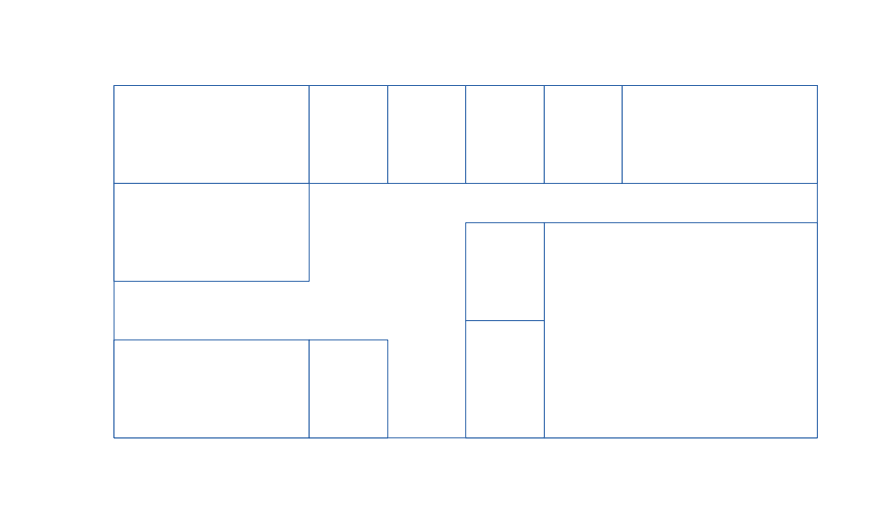
\includegraphics[width=.5\textwidth]{images/floorMap.png}
	\caption{Sample floor maps \parencite{mapCraft}}
	\label{fig:floorMaps}
\end{figure}

\paragraph{Beacon locations} are used to determine the position by measuring the distance to the beacons with the help of signal strength and multilateration. This method is unprecise. More accurate positioning is achieved in combination with fingerprinting. A map showing beacon positions is given in figure \ref{fig:beacon}.

\begin{figure}[h]
	\centering
		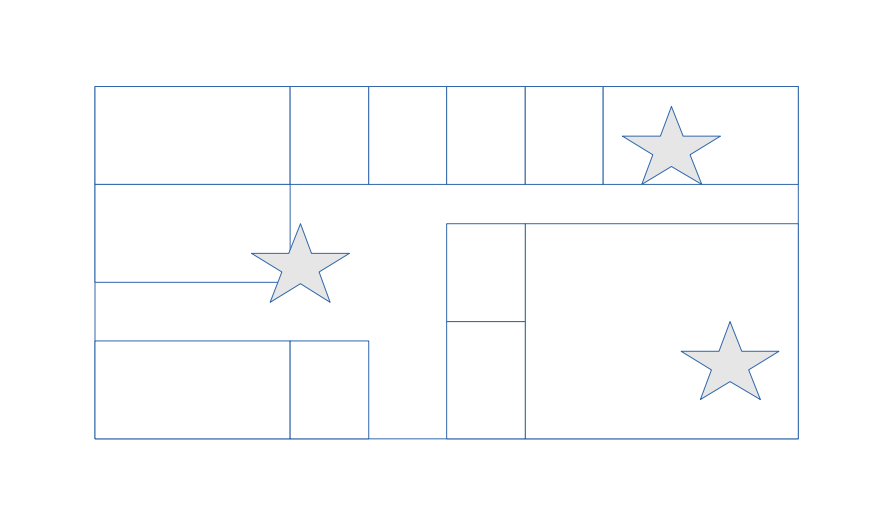
\includegraphics[width=.5\textwidth]{images/apLocations.png}
	\caption{Sample iBeacon locations \parencite{mapCraft}}
	\label{fig:beacon}
\end{figure}

\paragraph{Landmarks} function as extensions to floor maps due to the fact that a persons position can't intersect with landmarks \parencite{mapCraft}. This leads to more precise location determination. Furthermore landmarks are easy to spot and can be navigation destinations. A map including landmarks is shown in figure \ref{fig:landmarks}.

\begin{figure}[h]
	\centering
		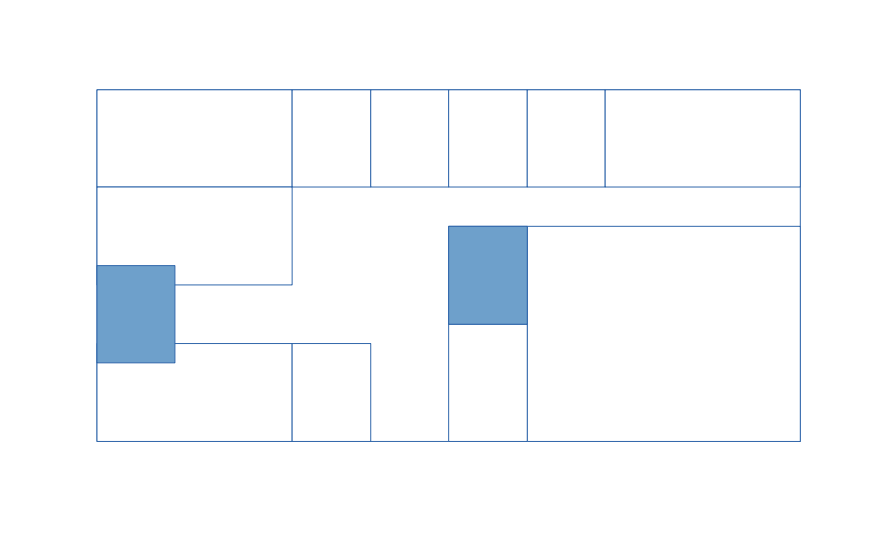
\includegraphics[width=.5\textwidth]{images/landmarks.png}
	\caption{Sample landmarks \parencite{mapCraft}}
	\label{fig:landmarks}
\end{figure}

\paragraph{Magnetic Flux Maps} are maps based on the fluctuation of magnetic fields influenced by obstructed metals. Flux maps store magnetic density fingerprints in $\mu T$ (Tesla) ranging from 25 to 65 $\mu T$ shown in figure \ref{fig:fluxMap} \parencite{fluxMap1}. 

\begin{figure}[h]
	\centering
		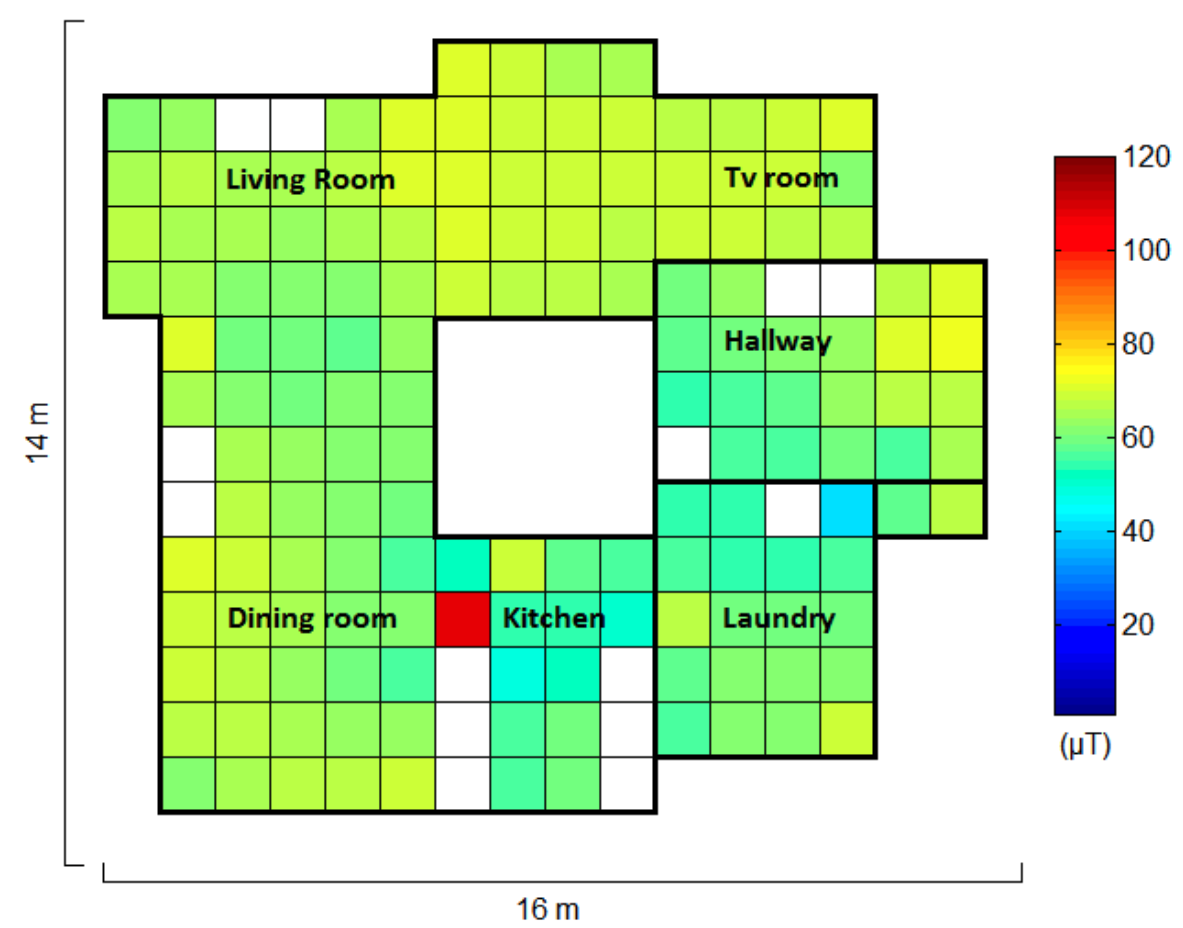
\includegraphics[width=.5\textwidth]{images/fluxMap.png}
	\caption{Sample flux map \parencite{fluxMap1}}
	\label{fig:fluxMap}
\end{figure}


\paragraph{WiFi, Blotooth or Zigbee Fingerprinting} based on measuring the intensity of the received signal analoge to magentic flux density maps with additional information about the device ID. These maps are referencing RSS-based localization where RSS means "Received signal strength". A sample map is shown in figure \ref{fig:intersection}. 

\begin{figure}[h]
	\centering
		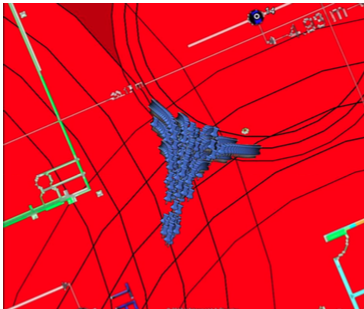
\includegraphics[width=.5\textwidth]{images/rangeIntersection.png}
	\caption{Intersection of accessspoint ranges including possible locations of the user (blue)}
	\label{fig:intersection}
\end{figure}

\paragraph{LED pattern map} is used to enable LED Pattern based positioning. The map stores the positions of all mounted LEDs in three dimension. Using the internal magnetometer and accelerometer as well as the angle of view the position can be calculated by patternmatching \parencite{bytelight}. 

\paragraph{Pedestrian Movement Model} In addition to all these maps pedestrian movement model could be used as constraint. Since this is one big area of research itself we are not discussing it in detail in this paper. However in general models of swarm computing could be applied for infrastructure mode systems - since humans are often behaving like a swarm of birds or ants. For independent mode a statistical model could be applied taking constraints like Landmarks and Floor-plans into account.  

As could be observed these different constraints are expecting different sensors as input. However redundant systems are known to guarantee a higher reliability. This brings up the topic of the next section: Sensor Fusion.

\pagebreak
\subsection{Sensor Fusion}
A comprehensive solution for indoor navigation should be able to combine different types of sensors. Sensor fusion was already mentioned 2008 by \textcite{dlrFiebig} as a essential part for future pedestian navigation systems.  
Sensor fusion could be done using different methods and algorithms. One prominent algorithm for example is the Kalman Filter that is used by the German Aerospace Center. Other algorithms that could be used are the Central Limit Theorem, Bayesian Networks or the Dempster-Shafer theory. These four methods are now explained shortly.

\paragraph{Bayesian Network} A Bayesian Network is a directed acyclic graph with nodes representing random variables and edges representing conditional dependencies. In case of sensor fusion one node would represent the result and other nodes the observed sensors influencing the result. Since the sensors are generating continuous instead of discrete random variables an approximating continuous model needs to be used.
In case of localization this does mean that it is assumed that the sensor measurements are conditionally independent of each other given the state (where the states represent user locations). This fact is visualized in figure \ref{fig:bayes}.
Then the problem of sensor fusion can be seen as: find $p(S_{t}| Z_{t}={z_{t}[0],z_{t}[1],...,z_{t}[n]})$ where $z$ are the positions given by different sensors, $S$ is the state and $t$ is the time \parencite{mapCraft}.

\begin{figure}[h]
	\centering
		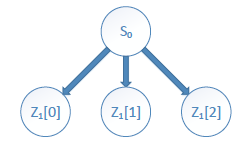
\includegraphics[width=.5\textwidth]{images/bayes.png}
	\caption{Sample Bayes model showing the independence of the measurements given the state.}
	\label{fig:bayes}
\end{figure}

Extending this model to a sequence of states linked through transition probabilities leads to recursive Bayesian models, such as Hidden Markov Models "where state variables are discrete, and the transition model $p(S_t|S_{t-1})$ is a matrix" \parencite{mapCraft}.

\paragraph{Kalman Filter} 
The location of the user is considered as a continuous variable and the filter relies on the Bayesian model. The Kalman Filter estimates the new position of a moving node by taking into account the old position - \textit{prior knowledge} of the state - and some internal sensor data - \textit{measurements}. 
The \textit{prior knowledge} of the state and reliable RSS Maps (Fingerprinting) are used to generate a \textit{prediction} of the next state - this prediction is defined by a Gaussian function. The (noisy) measurements itself are forming another Gaussian distribution. The fact that the product of two Gaussian functions is another Gaussian function is applied to generate the best estimate. Thus the Kalman Filter is differentiating explicitly between a State-model (including the constraints) and filtering. During filtering the measurements are all assumed to be mutually independent. This causes a problem of separating between measurement noise of the sensors and unmodelled dependencies. 
One Kalman Filter especially extended for localization is called Extended Kalman Filter. The real time sensor fusion system developed by the DLR is using a Kalman filter for the stride estimation, and fuses other sensors and maps at a higher-level with an own optimized algorithm \parencite{dlrFiebig}. (This "own" algorithm was not explained in the source.)
	\textit{Note: The Kalman Filter is not to complex to work on a real time system in Independent Mode (Active Sensor System) \parencite{dlrFiebig} and works well with low cost sensors often used in wearable devices.}
	
\paragraph{Central Limit Theorem}
The Central Limit Theorem generally states that a sequence of similar processes is Gaussian distributed. This statistical method thus can be applied for sensor fusion with unknown underlying distribution. The only conditions are that $n$ is large (rule of thumb is $n>30$) where n is the number of independent experiments (stages), in each stage the same experiment is executed and expectation and variance of all stages are equal \parencite{kloess}. Since for multiple sensors as sources not exactly the same experiment with the same expectation and variance can be assumed. However if the sensors are considered as independent, applying the condition of the Bayesian Network (that the sensor measurements are conditionally independent of each other given the previous state) - and no sensor is dominating the expectation - it can be assumed that $E(Z) = \mu = \mu_1 + \mu_2 + ... + \mu_n$ and the variance as $Var(Z) = \sigma^2 = \sigma^2_1 + \sigma^2_2 + ... + \sigma^2_n$ for the different sensors ($1$ to $n$).
Thus with preprocessed error corrected sensor data and if the user can tolerate some delay (time needed to perform $n>30$ measurements using $k$ sensors and $k<<n$) the theorem is a satisfying model. 

Not only sensor fusion, but software able to analyse and filter the raw sensor data is necessary to get useful data. This is discussed in the next Section.

\subsection{Error correction and Filtering} \label{sec:error}
It is no secret that there could be various measurement errors by each of the possible sensors. To reduce the amount of errors before the sensor data is used by the positioning system various filters could be applied. In this paper three of these possible filters are explained in detail, after classical mathematic error analysis is explained shortly.

\subsubsection{Error Analysis}
Error analysis can be applied to a series of measurements, thus to a random variable is used to calculate:

\begin{itemize}
	\item a mean value 
	\item the variance for individual measurements
	\item the variance, confidence interval and the uncertainty of measurement.
\end{itemize}

After these values have been calculated error propagation is of interest for all indirect measured value. Therefore law of error propagation (If $Z = f(X; Y)$ then $s_z = \sqrt{(f_x(\bar x; \bar y) s_x)^2 + (f_y(\bar x; \bar y) s_y)^2}$ and $\bar z = f(\bar x; \bar y)$ where $s$ is the corresponding standard deviation) can be applied, and in some cases the determination of a regression curve can help improving the measurement results \parencite{papula}. Especially for magnetometer, gyroscope, accelerometer and barometer error analysis including error propagation and regression is of interest. 

Error analysis can only be applied to random errors and not to systematic errors. Systematic errors exist if the measurement method is not completely reliable or the environment does not allow reliable measurements. The two filters described are an example on how to reduce systematic errors.

\subsubsection{Invalid Position Filter}
A correction filter that is implemented directly in the GPS Receiver is Invalid Position Filtering \parencite{mapCraft}. Every GPS position object is numerically flaged to be filtered out whenever certain circumstances apply. There are different vendors and different flags used to do so, common ones are for example the amount of satellites available for this position computation. If there are less than three satellites available the position obect is flaged as invalid. Other approaches verify whether the current position is too far away from the previous to be valid \parencite{mapCraft}. Objects which are flaged invalid are nullified and thus cannot be used from the host application. After beeing processed by the Invalid Position Filter the position objects are passed down the filterpipeline to the next available filter \parencite{mapCraft}. There have to be made considerations if this filter is to be implemented for different sensors since not every sensor is qualified to set usefull flags. Never the less Invalid Position Filters make sense for sensors calculating specific positions.


\subsubsection{Mask Filter} 
Deferred threshold levels for specific measurements are referred as masks \parencite{mapCraft}. Their purpuse is to eliminate GPS positions that do not meet certain quality standards defined through the masks. Examples are Position Dilution of Precision (PDOP), Signal to Noise ratio (SNR) and dimensions of the position (2D or 3D). Low values for PDOP or SNR combined with high treshold levels lead to rejection of the position, but do not neccessarily mean that the position is inaccurate, more that the chances for the position being accurate are low \parencite{mapCraft}. In other words nullification of positions that do not meet masks is undesirable. Considering the case that more and more sensor data gets low PDOPs or SNRs for whatever reason, this would lead to more rejection of positions. Unlike other error correction Filters, the threshold levels can be adjusted. Dynamic filtering of GPS positions are implemented in the Mask Filter. Meaning that the ratio of accepted versus rejected amounts of positions by the mask filter have an influence on the mask threshold levels \parencite{mapCraft}. Dynamic adjustments up to the point of disabling masks are made in order to remain at least few positions. "The motto here is that a bad position is better than no position"\parencite{mapCraft}. Hence Mask Filter are very simmilar to Invalid Position Filter.

The mask filter is eliminating systematic errors and is thus considerable for WiFi and Bluetooth signals.


\subsubsection{Map Matching}
The idea behind the map matching filter is to correct any position that does not match the rules of a map. Whenever an object to track with the help of GPS can be bound to a grid like system, map matching is used to determine the exact possible position in relation to the original gps data, cancelling out errors during GPS data gathering. This works with automobile navigation because the assumption that a car always has to travel on a particular road. Therefor the amount of possible positions for the car are shrunk down dramastically thus increasing the accuracy of tracking. On the other hand this rules for traffic cannot be easily transfered to pedestrian navigation system. The fact that people usually walk in wide spread areas without defined allignment or direction makes it nearly impossible to define routes of travel \parencite{mapCraft}. New strategys have to be developed. Due to the fact that pedestrians only can walk on pavement like underground the algorithm has to make assumptions about where the user can not be. Therefor excluding walls, lakes and other obstacles. Crosspassing walls is only possible by using doors, changing levels only by using elevators or stairs. All this areas are handled with lik "off-limits" where usually no pedestrian will be traveling. If any GPS position points on obstacles of either kind, it can be safely reasoned that the position must be inaccurate.

\paragraph{Particle Filter} 
There have to be taken multiple measurements when estimating position with the help of Particle Filters. The true position is estimated by combining these measurements. The concept behind the Particle Filter is to generate randomly distributed particles that represent positions in space.  First the distance to an object has to be derived from measurements (e.g. sonar). From all the distributed particles the algorithm selects only those particles that best match the measured distance to the object. Particles that match the measured distance live on while the others die away. The particles that match the measurements the closest are propaganding their position into the next iteration by spawning new particels around them. The more accurate the particles are to the real measurements the more are spawned around them in the next iteration. The second measurement is the true direction to an object. As in the distance measurement particles which match the true dirction closely live on the others die. Now both, distance and direction data is used to localize an agent in the system. the result is a cloud of particles which respresent the approximated true position. This cloud can be mapped to a single position by calculating the average of all particles. By using a system of marked obstacles in maps and map matching, Particle Filters seem to be a usefull extension to the that. Real world measurements like distance and direction can be taken into account and further on be used in Map Matching. 

\paragraph{Hidden Markov Model(HMM)}
The Hidden Markov Model is a statistical model based on a dynamic baysian network. The idea behind the HMM is a state based system where every state transition is random. Furthermore every transition has a probability depending on the current state. No history is involved. Additionaly these transition probabilitys are constant considering time. The state model is not known (hidden) whereas every state has its own emissions, outputs that occure with a certain probability. A sequence of emissions is used to jump to conclusions about the hidden state model. Yingjun Zhang et al used the Hidden Markov Model for pedestrian Navigation System in conjunction with MEMS Inertial Sensors, based on accelerometer and a special form of gyroscope with six degrees of freedom \parencite{HiddenMarkovModel}.


\paragraph{Dempster-Shafer Theory} is a framework for reasoning with uncertainty used to apply a mathematical theory of evidence. The theory is based on believes and plausibility. A Believe is a probability assigned to sets of possibilities. For example an agent being in an area (area would be a set op possible locations). The plausibility would be the sum of events which do not contradict the assumptions of believe - i.e. single measurements \parencite{reichardt}.

In case of map matching degrees of belief could be assigned to different locations based on sensor information and combined with the conditions provided by the map. 

\pagebreak